\newcommand{\econtexRoot}{.}

\documentclass[\econtexRoot/HAFiscal]{subfiles}
\onlyinsubfile{\externaldocument{\econtexRoot/HAFiscal}} % Get xrefs -- esp to apndx -- from main file; only works if main file has already been compiled

\begin{document}

\FloatBarrier
\hypertarget{robustness}{}\par\section{Robustness}
\notinsubfile{\label{sec:robustness}}

In this section, we analyze how sensitive our results are to some of the parameters in the model. In particular, we focus on parameters that heavily influence consumers' incentives to save. These parameters are (1) the interest rate that affects the returns on saving and (2) the degree of risk aversion and the replacement rates when unemployed with or without benefits that affect the strength of a precautionary saving motive. The aim is to alter these incentives while maintaining the requirement that the distributions of liquid wealth in each education group match the distributions in the data. Hence, in each case, we re-estimate the distributions of discount factors in each education group (and, if necessary, the degree of splurge spending in consumption). The aim is thus to compute new results for a model with different parameters that also fits data on the distribution of liquid wealth. At the end of the section, we also consider how changing the properties of the recession affects our main results. 

\hypertarget{changing-the-interest-rate}{}\par\subsection{Changing the interest rate}
\notinsubfile{\label{sec:robust_R}} 
In our baseline calibration, the interest rate is set to $1$ percent per quarter. Here, we consider the effect on our results of increasing or decreasing this value. Changes to the U.S. interest rate do not affect the estimation of the splurge parameter $\varsigma$. However, before we can calculate updated results for a different interest rate, the distribution of discount factors within each education group must be re-estimated for the model to continue to match the liquid wealth distributions. 

\subsubsection{Discount factor distributions with different interest rates}
\notinsubfile{\label{sec:robust_R_estim}}

Table~\ref{tab:robustness_R} shows the values we obtain for the discount factor distributions when we change the quarterly interest rate by either decreasing it to $0.5$ percent or increasing it to $1.5$ percent. In both cases, the estimation can exactly match the median liquid-wealth-to-permanent-income ratios for each education group reported in panel~B of table~\ref{tab:estimBetas}. 

\begin{table}[t]
	\begin{center}
		\begin{tabular}{lc|cccccc} 
			\toprule
			& & \multicolumn{2}{c}{Dropout} & \multicolumn{2}{c}{Highschool} & \multicolumn{2}{c}{College} \\ \midrule 
			& Splurge & $\beta$ & $\nabla$ & $\beta$ & $\nabla$ & $\beta$ & $\nabla$ \\ \midrule 
			$R = 1.005$ & 0.307 & 0.740 & 0.298 & 0.927 & $0.193^{*}$ & 0.989 & 0.0082 \\
			$R = 1.01$ (baseline) & 0.307 & 0.735 & 0.298 & 0.924 & $0.137^{*}$ & 0.984 & 0.0096 \\ 
			$R = 1.015$ & 0.307 & 0.724 & $0.357^{*}$ & 0.919 & $0.138^{*}$ & 0.979 & 0.0105 
			\\ \bottomrule 
		\end{tabular}
		\caption{Estimates of the splurge and $(\beta,\nabla)$ for each education group for different values of the interest rate $R$.
A $*$ denotes an estimate of $\nabla$ that implies that the largest discount factor value in our discrete approximation would violate the GIC and is thus replaced with a value below the upper bound.}
		\notinsubfile{\label{tab:robustness_R}}
	\end{center}
\end{table}

The first row of table~\ref{tab:robustness_R} shows the estimated $\beta_e$ and $\nabla_e$ for the lower interest rate of $0.5$ percent per quarter.
With a lower interest rate and an unchanged discount factor distribution, consumers would tend to substitute away from saving and toward current consumption.
They would therefore accumulate less wealth, leading to a lower median liquid-wealth-to-permanent-income ratio.
In all education groups, we therefore see that the estimated discount factor distributions are centered around higher values of $\beta$ to ensure that the model still matches the median liquid-wealth-to-permanent-income ratio in the data.
An increase in patience cancels out the effect of the lower interest rate on median saving.
Similarly, in the third row, we see the opposite effect when the interest rate is increased to $1.5$ percent.
Ceteris paribus saving would be more attractive with a higher interest rate, and this is offset by a reduction in $\beta$.


Figure~\ref{fig:LorenzPtsrobustnessR} in Appendix~\ref{app:DF_R} shows that the re-estimated model also matches the liquid wealth distributions for each of these values of the interest rate.
From table~\ref{tab:robustness_R}, we see that the values of $\nabla_e$ for the three education groups do not need to change much for this to be the case.



\subsubsection{Results with different interest rates}
\notinsubfile{\label{sec:robust_R_results}}

In this section, we repeat the welfare analysis conducted in section \ref{sec:welfare} for different values of the interest rate.
As in that section, the stimulus check and payroll tax cut policy have been adjusted to be of the same fiscal size as the UI extension.
All three policies are implemented during a recession.
We determine welfare results for the policies implemented both with and without aggregate demand effects.

As can be seen in table \ref{tab:robustness_R_results}, a higher interest rate increases the welfare benefits of all three policies.
This result obtains despite only small changes in the multipliers for the different interest rates.
Higher interest rates result in higher welfare benefits, as measured in lifetime consumption units, for all policies because the benefits of the policies (in the numerator) are front-loaded compared with a proportional increase in consumption through all periods (in the denominator).
Thus, increasing the interest rate---which is also the social planner's discount rate---reduces the value of a proportional increase in consumption by more than the consumption increases associated with each policy.
Nevertheless, the qualitative result that the extended UI benefits provide by far the highest welfare gains, followed by the stimulus checks, is strongly robust to changes in the interest rate.
%\footnote{The 10y-horizon multiplier of the policies increases by about 1 to 1.5 percent in moving from an interest rate of 1.01 (the baseline as reported in table \ref{tab:Multiplier}) to 1.015.}

\begin{table}[t]
	\begin{center}
		\begin{tabular}{@{}lllll@{}}
			\toprule
			&                    & Stimulus check & UI extension & Tax cut \\ \cmidrule(l){1-5} 
			\multirow{3}{*}{no AD effects}            	& $R = 1.005$ 			& 0.005        & 0.295       & 0.001	\\
			& $R = 1.01$ (baseline) & 0.011        & 0.509       & 0.002   	\\
			& $R = 1.015$ 			& 0.014        & 0.666       & 0.003   	\\ \cmidrule(l){1-5}
			\multirow{3}{*}{AD effects}					& $R = 1.005$    		& 0.081        & 0.618       & 0.030  	\\		
			& $R = 1.01$ (baseline) & 0.151        & 1.101       & 0.056   	\\
			& $R = 1.015$    		& 0.215        & 1.496       & 0.081    \\ \cmidrule(l){1-5} 
		\end{tabular}
		\caption{Consumption-equivalent welfare gains in basis points, calculated for policies implemented in a recession with and without aggregate demand effects, for different values of the interest rate $R$}
		\notinsubfile{\label{tab:robustness_R_results}}
	\end{center}
\end{table}


\FloatBarrier
\hypertarget{changing-risk-aversion}{}\par\subsection{Changing risk aversion} 
\notinsubfile{\label{sec:robust_gamma}} 

In our baseline calibration, consumers have a risk aversion of $\gamma=2$, which is quite common in macroeconomic models.
Here, we investigate how alternative values of $\gamma$ would influence our results.
Again, we re-estimate the distribution of discount factors within each education group, but in this case, we also re-estimate the degree of splurge spending in consumption.


\subsubsection{Discount factor distributions with different risk aversion}
\notinsubfile{\label{sec:robust_gamma_estim}}

Table~\ref{tab:robustness_gamma} displays the values we obtain for the splurge and the discount factor distributions when we change $\gamma$ to $1$ and $3$.
The table shows that the splurge is not very sensitive to the degree of risk aversion.
The splurge controls the degree of spending that consumers do before considering the trade off involved in optimally allocating spending over time and across different future states of the world.
Risk aversion affects that trade off but does not have a big influence on a parameter that controls spending that is independent of that problem.


\begin{table}[t]
  \begin{center}
    \begin{tabular}{lc|cccccc} 
      \toprule
      & & \multicolumn{2}{c}{Dropout} & \multicolumn{2}{c}{Highschool} & \multicolumn{2}{c}{College} \\ \midrule 
      & Splurge & $\beta$ & $\nabla$ & $\beta$ & $\nabla$ & $\beta$ & $\nabla$ \\ \midrule 
      $\gamma = 1.0$ & 0.312 & 0.692 & 0.333 & 0.966 & $0.154^{*}$ & 1.05\textsuperscript{\textdagger} & 0.015 \\ 
      $\gamma = 2.0$ (baseline) & 0.306 & 0.735 & 0.298 & 0.924 & $0.137^{*}$ & 0.984 & 0.0096 \\
      $\gamma = 3.0$ & 0.304 & 0.593 & $0.459^{*}$ & 0.889 & 0.110 & 0.973 & 0.017 
      \\ \bottomrule 
    \end{tabular}
    \caption{Estimates of the splurge and $(\beta,\nabla)$ for each education group for different values of risk aversion, $\gamma$.
A $*$ denotes an estimate of $\nabla$ that implies that the largest discount factor value in our discrete approximation would violate the GIC and is thus replaced with a value below the upper bound.
A \textdagger\hspace{.01cm} indicates an estimate of $\beta$ that is so large that all values in the discrete approximation violate the GIC and replaced with a value below the upper bound.
    }
    \notinsubfile{\label{tab:robustness_gamma}}
  \end{center}
\end{table}

The second and third rows of table~\ref{tab:robustness_gamma} show results when we increase risk aversion from $\gamma=2.0$ to $\gamma=3.0$.
Increasing risk aversion for all types within an education group makes the precautionary saving motive stronger for all consumers in that group.
Ceteris paribus, these consumers would then increase the amount of liquid wealth they accumulate, and the median liquid-wealth-to-permanent-income ratio for the education group would increase.
For all the education groups, the discount factor distributions are therefore centered around lower values of $\beta$ when risk aversion is increased to $3.0$.
As for the increase in the interest rate in section~\ref{sec:robust_R_estim}, the decrease in patience counteracts the stronger incentive to save from the higher risk aversion.
However, the reductions in $\beta$ when increasing risk aversion from $2.0$ to $3.0$ are much larger than when increasing the interest rate from $1$ to $1.5$ percent.


The effects on $\nabla$ and the concentration of the liquid wealth distribution may be less intuitive.
However, if the only changes were to increase risk aversion and to decrease $\beta$ while keeping $\nabla$ fixed at the value for $\gamma=2.0$, then the result would be a liquid wealth distribution that was much less concentrated than in the data.
If all consumers in an education group are less patient, the reduction in saving is larger for the wealthier consumers.
Thus, to maintain the concentrated wealth distribution, $\nabla$ increases substantially for the Dropout and College groups.
The results are distributions of discount factors within these groups that are centered around lower values, but that are much more dispersed.
The effect is that the discount factor for the most patient type within each education group is not changed very much, but the lowest discount factor is much lower than when $\gamma=2.0$, and the liquid wealth distributions remain as concentrated as they are in the data.

For the Highschool group the effect is a bit different.
In the baseline case, $\nabla_h$ is so high that the discount factor for the most patient type violates the GIC.
The discount factor for the most patient type is therefore not determined by $\nabla_h$.
When risk aversion is increased to $\gamma=3.0$ and the discount factor distribution is centered around a lower value for $\beta_h$, the estimated value of $\nabla_h$ no longer implies that the GIC is violated by the most patient type.
Thus the comparison of $\nabla_h$ with the value from the baseline is not so relevant.\footnote{Note that with risk aversion set to $\gamma=3.0$, the discount factor for the most patient type in the Dropout group is also constrained by the GIC.}

When we decrease risk aversion to $\gamma=1.0$, however, we run into problems when estimating the discount factor distribution.
Our model fails to jointly fit both the median liquid-wealth-to-permanent income ratios and the liquid wealth distributions for the Dropout and the College groups.
Table~\ref{tab:robustness_gamma_mlwpi} shows that for $\gamma=1.0$, while the model can match the median liquid-wealth-to permanent-income ratios for the Highschool and College groups, it does not do so for the Dropout group.
With such a low value of risk aversion, the estimation cannot yield a discount factor distribution where the median household has any significant savings.
Instead, the resulting distribution concentrates most of the saving with the most patient types so that the distribution of liquid savings is matched fairly well.
This is shown in the upper left panel of Figure~\ref{fig:LorenzPts_robustness_CRRA}.


For the College group we encounter a different problem.
With a lower risk aversion and a weaker precautionary saving motive the intuition from the case where $\gamma=3.0$ is reversed.
When households are less risk averse, the model requires them to be more patient to match the same level of saving as in the baseline case.
But the estimated values of $\beta_c$ and $\nabla_c$ in Table~\ref{tab:robustness_gamma} yield a discount factor distribution that violates the GIC for all the 7 types.
Their discount factor is then set to a value close to the upper bound which is estimated to fit the overall level of saving.
As row~1 of Table~\ref{tab:robustness_gamma_mlwpi} shows, the model then fits the median liquid wealth to permanent income ratio.
However, the lower left panel of Figure~\ref{fig:LorenzPts_robustness_CRRA} shows that without dispersion of the discount factors for this education group, the model does not match the distribution of liquid wealth.

 
\begin{table}[th]
  \begin{center}
    \begin{tabular}{lccc}
      \multicolumn{4}{l}{} \\ \midrule
      & Dropout & Highschool & College \\ \midrule
      Median LW/PI (data, percent) & 4.64 & 30.2 & 112.8 \\ 
      Median LW/PI (model, $\gamma = 1.0$, percent) & 0.00 & 30.1 & 112.8 \\	
      Median LW/PI (model, $\gamma = 2.0$, percent) & 4.64 & 30.2 & 112.8 \\
      Median LW/PI (model, $\gamma = 3.0$, percent) & 4.64 & 30.2 & 112.8 \\ \bottomrule
    \end{tabular}
    \caption{Median liquid-wealth-to-permanent-income ratios}
    \notinsubfile{\label{tab:robustness_gamma_mlwpi}}	
    \parbox{15cm}{\small \vspace{.05cm} \textbf{Note}: The table shows the weighted median ratio of liquid-wealth-to permanent-income from the 2004 SCF and in versions of the model with different risk aversion.
In the annual data from the SCF, the annual PI is divided by 4 to obtain a quarterly number.\normalsize}
  \end{center}
\end{table}

\begin{figure}[th]
  \begin{center}
    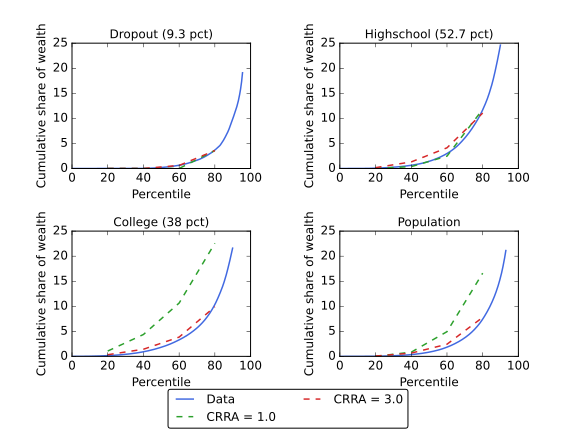
\includegraphics[width=.9\textwidth]{../Figures/LorenzPoints_robustness_CRRA}
    \caption{Distributions of liquid wealth within each educational group and for the whole population from the 2004 Survey of Consumer Finances and from the estimated model for different values of risk aversion, $\gamma$}
    \notinsubfile{\label{fig:LorenzPts_robustness_CRRA}}
  \end{center}
\end{figure}

The strength of the precautionary saving motive is determined by more than just risk aversion.
The risks that households face also drive the strength of this motive for saving, and in our model, a key risk is unemployment risk.
The replacement rates that households face when they are unemployed with or without benefits play an important role.
In section~\ref{sec:robust_benefits}, we therefore consider an alternative calibration of these values.


\subsubsection{Results with different risk aversion}
\notinsubfile{\label{sec:robust_gamma_results}}

In this section, we conduct the welfare analysis for the case with $\gamma=3.0$.
We do not repeat these calculations for $\gamma=1.0$, since in that case the model cannot match the level and distribution of liquid wealth making the results for that case less interesting.


A higher risk aversion implies a greater welfare loss associated with the same drop in consumption, and thus, a greater welfare gain for policies that reduce the consumption drop.
However, changing the risk-aversion parameter has a number of other ramifications for our welfare measure that are difficult to assess without simulation.
A higher risk aversion (ceteris paribus) induces agents to hold a higher buffer stock of savings, making them less sensitive to adverse economic shocks in terms of their consumption response.
As argued earlier, and since we target the empirical wealth-to-income ratios, we increase impatience to counteract this larger incentive to save.
These changes then affect the consumption response of agents to the recession and to the policies implemented.


Table \ref{tab:robustness_gamma_results} shows the welfare results for the baseline case and for the higher value of risk aversion.
For $\gamma=3$ and AD effects switched on, we obtain slightly higher welfare effects than in the baseline.
When AD effects are switched off, this only applies in the case of the UI extension.
For both cases, with and without AD effects, the changes are quite small in magnitude.\footnote{Mirroring the welfare results, the 10y-horizon multipliers of the policies for the higher risk aversion value are very close to those for the baseline calibration.} Most importantly, the welfare ranking of the policies is robust to this alternative value for the risk-aversion parameter.

\begin{table}[]
  \begin{center}
    \begin{tabular}{@{}lllll@{}}
      \toprule
      &                    & Stimulus check & UI extension & Tax cut \\ \cmidrule(l){1-5} 
      \multirow{2}{*}{no AD effects}
      & $\gamma = 2.0$ (baseline) & 0.011          & 0.509        & 0.002   \\
      & $\gamma = 3.0$ 			& 0.011          & 0.558        & 0.002   \\ \cmidrule(l){1-5} 
      \multirow{2}{*}{AD effects}
      & $\gamma = 2.0$ (baseline) & 0.151          & 1.101        & 0.056   \\
      & $\gamma = 3.0$    		& 0.156          & 1.207        & 0.059   \\ \cmidrule(l){1-5} 
    \end{tabular}
    \caption{Consumption-equivalent welfare gains in basis points, calculated for policies implemented in a recession with and without aggregate demand effects, for different values of risk aversion, $\gamma$}
    \notinsubfile{\label{tab:robustness_gamma_results}}
  \end{center}
\end{table}



\hypertarget{changing-benefits}{}\subsection{Changing benefits} 
\notinsubfile{\label{sec:robust_benefits}} 

In our baseline calibration, we follow \cite{rothstein2017scraping} and calibrate the replacement rates to $\rho_b=0.7$ with unemployment benefits and $\rho_{nb}=0.5$ without benefits.
Here, we consider replacement rates that are considerably less generous and more in line with values used in the previous macro literature with unemployment in models with heterogeneous agents.
The alternative values we consider are a replacement rate of $\rho_{b}=0.3$ when unemployed with benefits, as in \cite{carroll2020modeling}, and a replacement rate of $\rho_{nb}=0.15$ when unemployed without benefits.
This latter value is the same as the replacement rate used in \cite{den2010computational}.\footnote{In \cite{den2010computational}, there is only one unemployment state and, hence, no sense in which benefits expire after a while.
Therefore, this replacement rate applies for long-term unemployed, as it does in our model, but in this paper there is also an intermediate state in which benefits are higher until they expire.} With these replacement rates, being unemployed is more serious for consumers than in our baseline calibration, and the precautionary saving motive is stronger.


\subsubsection{Discount factor distributions with different benefits}
\notinsubfile{\label{sec:robust_benefits_estim}}

Table~\ref{tab:robustness_benefits} shows that when benefits are less generous and the precautionary motive is stronger, the estimated discount factor distributions are centered on lower values of~$\beta$.
The intuition is similar to the case when increasing risk aversion from $\gamma=2.0$ to $\gamma=3.0$, discussed in section~\ref{sec:robust_gamma_estim}: A stronger precautionary motive for saving must be counteracted by a lower average discount factor to match the same average level of saving as before.
The distributions must also be more dispersed to match the same concentration of liquid wealth.\footnote{Note that the estimated $\nabla_h$ values for the Highschool group are not directly comparable in terms of the degree of dispersion.
One of these estimate is affected by hitting the GIC-imposed upper bound, but the other is not.} In fact, the estimated discount factor distributions for the alternative calibration of the replacement rates are very similar to those reported for $\gamma=3.0$ in row~3 of table~\ref{tab:robustness_gamma}.


\begin{table}[t]
  \begin{center}
    \begin{tabular}{llc|cccccc} 
      \toprule
      & & & \multicolumn{2}{c}{Dropout} & \multicolumn{2}{c}{Highschool} & \multicolumn{2}{c}{College} \\ \midrule 
      & & Splurge & $\beta$ & $\nabla$ & $\beta$ & $\nabla$ & $\beta$ & $\nabla$ \\ \midrule 
      Baseline & ($\rho_{b}=0.7$, $\rho_{nb}=0.5$) & 0.306 & 0.735 & 0.298 & 0.924 & $0.137^{*}$ & 0.984 & 0.010 \\ 
      Altern. & ($\rho_{b}=0.3$,  $\rho_{nb}=0.15$) & 0.306 & 0.609 & $0.445^{*}$ & 0.890 & 0.116 & 0.978 & 0.016
      \\ \bottomrule 
    \end{tabular}
  \end{center}
  \caption{Estimates of the Splurge and $(\beta,\nabla)$ for each education group for the baseline replacement rates $\rho_{b}$ and $\rho_{nb}$ and an alternative calibration.
A $*$ denotes an estimate of $\nabla$ that implies that the largest discount factor value in our discrete approximation would violate the GIC and is thus replaced with a value below the upper bound.}
  \notinsubfile{\label{tab:robustness_benefits}}
\end{table}


\FloatBarrier
\subsubsection{Results with different benefits}
\notinsubfile{\label{sec:robust_benefits_results}}

In this section, we perform the welfare analysis for different benefit replacement rates.
Table \ref{tab:robustness_benefit_results} shows that the alternative parameterization of the unemployment replacement rates yields considerably higher welfare benefits for the UI extension policy.
In particular, the lower the replacement rate under the no-benefit regime, the more harmful is the expiration of eligibility to the UI.
The UI extension is thus particularly powerful if $\rho_{nb}$ is small, which is mirrored by the 10y-horizon multiplier of the UI extension policy.
It increases from 1.20 in the baseline calibration to 1.38 under the lower replacement rates.
In contrast, multipliers and welfare effects of the other two policies do not change dramatically under the alternative calibration.
Again, our ranking of the three policies remains the same.


\begin{table}[]
  \begin{center}
    \begin{tabular}{@{}lllll@{}}
      \toprule
      &                    & Stimulus check & UI extension & Tax cut \\ \cmidrule(l){1-5} 
      \multirow{2}{*}{no AD effects} 	& Baseline  ($\rho_{b}=0.7$, $\rho_{nb}=0.5$) 		& 0.011          & 0.509        & 0.002   \\
      & Altern.  ($\rho_{b}=0.3$, $\rho_{nb}=0.15$) 	& 0.043          & 1.845        & 0.003   \\ \cmidrule(l){1-5} 
      \multirow{2}{*}{AD effects}		& Baseline  ($\rho_{b}=0.7$, $\rho_{nb}=0.5$)    	& 0.151          & 1.101        & 0.056   \\
      & Altern.  ($\rho_{b}=0.3$, $\rho_{nb}=0.15$)    & 0.157          & 2.514        & 0.048   \\ \cmidrule(l){1-5} 
    \end{tabular}
    \caption{Consumption equivalent welfare gains in basis points, calculated for policies implemented in a recession with and without aggregate demand effects, for different unemployment benefit rates}
    \notinsubfile{\label{tab:robustness_benefit_results}}
  \end{center}
\end{table}




\FloatBarrier
\hypertarget{changing-the-properties-of-the-recession}{}\par\subsection{Changing the properties of the recession}

In this section, we alter two properties of the recession and study the effect of those changes (one at a time) on our main results.
First, we lower the average length of a recession from six quarters in the baseline to four quarters.
Second, we increase the consumption elasticity of the aggregate demand effect, $\kappa$, from 0.3 in the baseline to 0.5.
In either case, the parameter changes do not require a re-estimation of the discount factor distribution, since the baseline saving behavior is unaffected by properties of the recession, which arrives as an MIT shock.


Table \ref{tab:robustness_recession_property_results} presents the welfare results for different properties of the recession.
In case of a shorter average recession length of four, instead of six, quarters, we observe lower welfare effects of the policies.
As argued earlier, the reason is that the policies are particularly effective during recessions.
With a shorter average recession length, the additional spending induced by the policies is now less likely to occur while the recession is ongoing.
This outcome can also be seen by investigating the 10y-horizon multipliers of the policies, which fall slightly for all three policies considered: from 1.245 in the baseline to 1.224 in case of the shorter recession length for the stimulus check, from 1.200 to 1.180 for the UI extension, and from 0.999 to 0.967 for the tax cut.

A higher value for $\kappa$---and hence stronger aggregate demand effects---considerably increases the welfare effects of each policy.
Of course, this is only the case in the version of the model where the aggregate demand effects are active.
In their absence, there is no change in the welfare results relative to the baseline calibration.
The larger $\kappa$ implies a larger boost to aggregate income in response to the demand effects of the policies.
This larger boost translates to a larger increase in consumption and thus a stronger welfare effect.
Under stronger AD effects, the policies also have considerably larger 10y-horizon multipliers.
The stimulus check exhibits a multiplier of 1.636 (baseline: 1.245); the UI extension, a multiplier of 1.492 (1.200); and the tax cut, a multiplier of 1.152 (0.999).


\begin{table}[]
  \begin{center}
    \begin{tabular}{@{}lllll@{}}
      \toprule
      &                    											& Stimulus check & UI extension & Tax cut 	\\ \cmidrule(l){1-5}
      \multirow{2}{*}{no AD effects} 					& Baseline 						& 0.011          & 0.509        & 0.002   	\\ 
      & Shorter average recession, 4q & 0.010          & 0.424        & 0.002  	\\
      & Stronger AD effects, 0.5 		& 0.011          & 0.509        & 0.002   	\\ \cmidrule(l){1-5}
      \multirow{2}{*}{AD effects}						& Baseline    					& 0.151          & 1.101        & 0.056   	\\
      & Shorter average recession, 4q & 0.143          & 0.926        & 0.045   	\\
      & Stronger AD effects, 0.5    	& 0.297          & 1.695        & 0.110   	\\ \cmidrule(l){1-5} 
    \end{tabular}
    \caption{Consumption-equivalent welfare gains in basis points, calculated for policies implemented in a recession with and without aggregate demand effects, for different properties of the recession}
    \notinsubfile{\label{tab:robustness_recession_property_results}}
  \end{center}
\end{table}


\FloatBarrier
%\hypertarget{changing-the-splurge}{}\par\subsection{Changing the splurge}
%
%In this last robustness section, we set the splurge factor to zero. As a consequence, the entirety of consumption is optimization-based.
%
%We re-estimate the discount factor distribution in the absence of the splurge. The model is able to replicate the distribution of liquid wealth within the education groups and for the population as a whole also in the absence of the splurge factor. However, the MPC falls significantly for all agents in the model. This is also evident from the 10y-horizon multipliers of the policies. For the stimulus check we obtain an 10y-horizon multiplier of 1.14 (1.339 in the baseline with the splurge), for the UI extension 1.22 (1.275) and for the payroll tax cut of 1.0 (1.079). Hence, the absence of the splurge particularly alters the multiplier value for the check and tax cut policy. The UI extension is less affected since it is targets only high MPC households, who also in the absence of the splurge spend much of the additional income quickly. 
%
%The welfare implications of the splurge removal are illustrated in Table \ref{tab:robustness_benefit_splurge}. Overall, the welfare benefit of the policies is reduced when agents do not splurge in response to the additional income provided. However, the welfare ranking of the three policies is unaffected by the removal of the splurge. 
%
%\begin{table}[]
%	\begin{center}
%		\begin{tabular}{@{}lllll@{}}
%			\toprule
%			&                    & Stimulus check & UI extension & Tax cut \\ \cmidrule(l){1-5} 
%			\multirow{2}{*}{no AD effects} 	& Baseline  (splurge = 0.307) 		& 0.011          & 0.580        & 0.002   \\
%			& Altern.  (splurge = 0) 	  & 0.010  & 0.470  & 0.002     \\ \cmidrule(l){1-5} 
%			\multirow{2}{*}{AD effects}		& Baseline (splurge = 0.307)    	& 0.171          & 1.266        & 0.065   \\
%			& Altern.  (splurge = 0)   & 0.113  & 1.098  & 0.052    \\ \cmidrule(l){1-5} 
%		\end{tabular}
%		\caption{Consumption equivalent welfare gains in basis points, calculated for policies implemented in a recession with and without aggregate demand effects, for different splurge values}
%		\notinsubfile{\label{tab:robustness_benefit_splurge}}
%	\end{center}
%\end{table}
%
%

\hypertarget{summary-of-robustness-exercises}{}\par\subsection{Summary of robustness exercises}
\notinsubfile{\label{sec:robust_summary}}

The robustness checks in this section show that our main results are robust to a wide range of alternative parameter choices.
A key step in the robustness exercises that directly affect the strength of the precautionary savings motive---changing the interest rate, the risk aversion parameter, or the replacement rates in the unemployment system---is to reestimate the distribution of discount rates.
Thus, we aim to match the distribution of liquid wealth in each case.
This appears to more or less pin down the aggregate consumption properties for the model, regardless of the other parameters.
Importantly, none of the robustness checks alter the ranking of policies in terms of their effectiveness and therefore the overall conclusions of this paper are unaffected.

Characteristics of the recession do, however, matter for our results.
Shorter recessions or those with smaller aggregate demand effects reduce the effectiveness of policies.
Conversely, more severe recessions will render the policies even more efficient than our baseline results suggest.

\ifthenelse{\boolean{Web}}{}{
  \end{document} \endinput
}
